%% LyX 2.3.3 created this file.  For more info, see http://www.lyx.org/.
%% Do not edit unless you really know what you are doing.
\documentclass{article}
\usepackage[T1]{fontenc}
\usepackage[utf8]{inputenc}
\usepackage{float}
\usepackage{booktabs}
\usepackage{amsmath}
\usepackage{graphicx}
\usepackage{microtype}
\usepackage[unicode=true,
 bookmarks=false,
 breaklinks=false,pdfborder={0 0 1},backref=section,colorlinks=false]
 {hyperref}

\makeatletter

%%%%%%%%%%%%%%%%%%%%%%%%%%%%%% LyX specific LaTeX commands.
%% Because html converters don't know tabularnewline
\providecommand{\tabularnewline}{\\}

%%%%%%%%%%%%%%%%%%%%%%%%%%%%%% User specified LaTeX commands.
\usepackage[final]{nips_2017}
% allow utf-8 input
% use 8-bit T1 fonts
% hyperlinks
\usepackage{url}% simple URL typesetting
\usepackage{booktabs}% professional-quality tables
\usepackage{amsfonts}% blackboard math symbols
\usepackage{nicefrac}% compact symbols for 1/2, etc.
% microtypography
\title{Trajectory Optimization with Dynamic Obstacles Avoidance}

\author{
  Philippe Weingertner and Minnie Ho\\
  \texttt{pweinger@stanford.edu minnieho@stanford.edu} \\
  %% examples of more authors
  %% \And
  %% Coauthor \\
  %% Affiliation \\
  %% Address \\
  %% \texttt{email} \\
  %% \AND
  %% Coauthor \\
  %% Affiliation \\
  %% Address \\
  %% \texttt{email} \\
  %% \And
  %% Coauthor \\
  %% Affiliation \\
  %% Address \\
  %% \texttt{email} \\
  %% \And
  %% Coauthor \\
  %% Affiliation \\
  %% Address \\
  %% \texttt{email} \\
}

\usepackage{algorithm,algpseudocode}


\usepackage{tikz}
\usetikzlibrary{shapes, arrows}
\usetikzlibrary{er,positioning}
\usetikzlibrary{matrix}
\tikzset{
    events/.style={ellipse, draw, align=center},
}

\usepackage{graphicx}
\usetikzlibrary{fit}
\usetikzlibrary{bayesnet}
\usepackage{pgfplots}

\usepackage{forest}


\usepackage{mathbbol}
 
\usepackage{listings}
\usepackage{xcolor}
 
\definecolor{codegreen}{rgb}{0,0.6,0}
\definecolor{codegray}{rgb}{0.5,0.5,0.5}
\definecolor{codepurple}{rgb}{0.58,0,0.82}
\definecolor{backcolour}{rgb}{0.95,0.95,0.92}
 
\lstdefinestyle{mystyle}{
    backgroundcolor=\color{backcolour},   
    commentstyle=\color{codegreen},
    keywordstyle=\color{magenta},
    numberstyle=\tiny\color{codegray},
    stringstyle=\color{codepurple},
    basicstyle=\ttfamily\footnotesize,
    breakatwhitespace=false,         
    breaklines=true,                 
    captionpos=b,                    
    keepspaces=true,                 
    numbers=left,                    
    numbersep=5pt,                  
    showspaces=false,                
    showstringspaces=false,
    showtabs=false,                  
    tabsize=2
}
 
\lstset{style=mystyle}

\makeatother

\begin{document}
% \nipsfinalcopy is no longer used

\maketitle
\begin{abstract}
We study the problem of Trajectory Optimization for Autonomous Driving
where we derive a motion plan on a pre-defined path. The challenge
is to avoid ten vehicles crossing our path, optimizing efficiency
and comfort, while making decisions in real-time. As part of a Model
Predictive Control (MPC) setup, we propose a Collision Avoidance model
based on an Elastic Model handling disjunctive constraints. We investigate
different optimization algorithms: Interior Point methods and adaptation
of a simplex algorithm to a problem initially defined over a quadratic
cost function. We provide reference implementations of the MPC setup,
Collision Avoidance Model and a fully custom solver. Finally we benchmark
and demonstrate the efficiency of our collision avoidance model, both
in terms of accuracy and real-time performances, on a serie of 100
randomly generated tests.
\end{abstract}

\section{Introduction}

This project  investigates trajectory optimization \cite{1986asdy.conf....3H}
in the presence of obstacles \cite{article,Fan2018BaiduAE,Katrakazas2015RealtimeMP,Zhang2020OptimizationBasedCA}.
One such application for this class of problems is that of autonomous
driving, where we have an ego vehicle and dynamic obstacles (vehicles,
pedestrians) which may intersect our desired trajectory and which
we wish to avoid using motion planning and control. 

\begin{figure}[H]
\noindent \begin{centering}
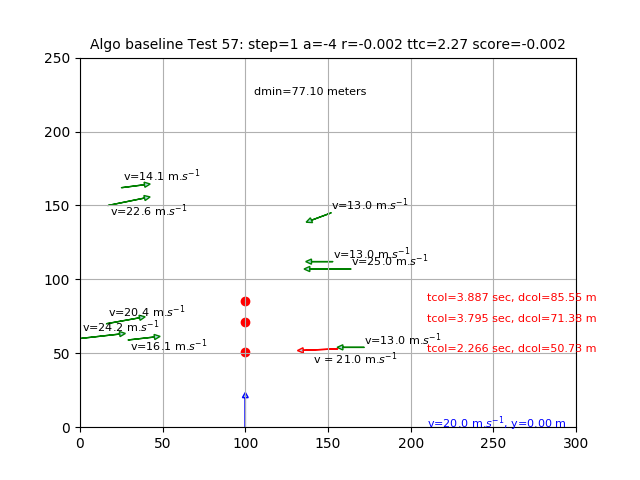
\includegraphics[scale=0.31]{img/test57}
\par\end{centering}
\caption{Collision Avoidance Tests Setup}
\end{figure}

Trajectory optimization minimize a cost function which takes into
account start and terminal states, as well as cost along the trajectory
path. The design space is subject to constraints on the states and
control input at sampled time points.

\section{Related Work}

A detailed survey of Motion Planning techniques for Autonomous Driving
is provided in \cite{7490340,Katrakazas2015RealtimeMP}. In order
to enable real-time applicability, the problem is typically decomposed
in a two-stage process. First a path is planned and then a Motion
Plan is derived over this pre-defined path (or over a set of pre-defined
paths). This strategy has been in use since the DARPA challenge \cite{article,Ferguson2009MotionPI,article0,article1}.
Path planning typically relies on search algorithms (A{*}, D{*}, RRT{*}
...) \cite{inproceedings,5980223} while the derivation of a Motion
Plan over a Path typically relies on either pre-computed velocity
profiles or solving online an Optimal Control problem. While MPC is
well established for pure trajectory tracking \cite{article2}, assuming
there exists a collision-free trajectory we want to follow, it can
also be used to derive a collision-free trajectory. In the first case,
a more complex and non linear vehicle dynamics model is used, while
in the second case, a linear approximation of the dynamics is used,
to quickly come up with a collision-free trajectory proposal. This
collision-free trajectory is then further refined in terms of comfort
and vehicle dynamics feasibility. 

We focus on the Motion Planning problem where a path is pre-defined
and we want to derive a collision-free trajectory considering a linear
approximation of the vehicle dynamics. There are several publications
on this subject \cite{7995713,Fan2018BaiduAE,7353382}, investigating
the use of MPC to derive a collision-free velocity profile. But they
assume that a higher level planner has already decided whether we
have to proceed or yield the way w.r.t. any other vehicle crossing
our path. While this may be a reasonable strategy when dealing with
a single or two objects crossing our path, we would like to scale
to multiple crossing objects. We would like to decide individually
and optimally w.r.t. every crossing object, wether we should proceed
or yield the way. This should be part of the optimization problem. 

\section{Problem Formulation}

We define a MPC problem over 20 time steps of $250$ ms each\textbf{
}with a Quadratic Cost function with $x\in\mathbb{R}^{60}$ and $160$
constraints. We have $120$ linear and nonlinear ($\left\Vert x_{\text{ego}}-x_{\text{obj}}\right\Vert \geq d_{\text{saf}}$)
inequality constraints and  $40$ linear equality constraints (Dynamics
Model). 

$\text{subject to }\begin{cases}
x_{k,\text{min}}\leq x_{k}\leq x_{k,\max}\\
u_{k,\text{min}}\leq u_{k}\leq u_{k,\max}\\
x_{k+1}=A_{d}x_{k}+B_{d}u_{k}\\
x_{0}=x_{\text{init}}\\
\forall\left(t_{\text{col}},s_{\text{col}}\right)_{i\in\left[1,10\right]} & x_{t_{\text{col}}^{\left(i\right)}}\left[1\right]<s_{\text{col}}^{\left(i\right)}-\Delta_{\text{safety}}\text{ or }x_{t_{\text{col}}^{\left(i\right)}}\left[1\right]>s_{\text{col}}^{\left(i\right)}+\Delta_{\text{safety}}
\end{cases}$

We wan't to avoid up to $10$ vehicles crossing our path. Spatio-temporal
collision points $\left(t_{\text{col}},s_{\text{col}}\right)$ are
defined with an associated uncertainty area $t_{\text{col}}\pm250\ ms,\ s_{\text{col}}\pm\Delta_{\text{safety}}$

We use linear dynamics model: with Constant Acceleration in between
2 time steps

\[
\begin{bmatrix}s\\
\dot{s}
\end{bmatrix}_{k+1}=A_{d}\begin{bmatrix}s\\
\dot{s}
\end{bmatrix}_{k}+B_{d}\begin{bmatrix}\ddot{s}\end{bmatrix}_{k}\text{with }A_{d}=\begin{bmatrix}1 & \Delta t\\
0 & 1
\end{bmatrix},B_{d}=\begin{bmatrix}\frac{\Delta t^{2}}{2}\\
\Delta t
\end{bmatrix}
\]


\section{Methods }

\subsection{Collision Avoidance Model}

We reformulate the collision avoidance model and later on demonstrate
the improvements it provides in a set of benchmarks. An implementation
of this model is available in \href{https://github.com/PhilippeW83440/AA222_Project/blob/master/itsc/mpc_mip.jl}{mpc\_mip.jl}. 

\subsubsection{Disjunctive Constraints}

In general the collision avoidance constraint is defined as $\left\Vert \text{pos}_{\text{ego}}-\text{pos}_{\text{obj}}\right\Vert _{2}\geq\text{d}_{\text{safety}}$ 

When considering the evolution of an ego vehicle along a path denoted
by $s\left(t\right)$ and a crossing-point for some other vehicle,
at $\left(t_{\text{cross}},s_{\text{cross}}\right)$, the collision
avoidance constraint is reformulated as: $\left|s\left(t_{\text{cross}}\right)-s_{\text{cross}}\right|\geq\text{d}_{\text{safety}}$.
Which is equivalent to a disjunctive constraint:

\[
s\left(t_{\text{cross}}\right)\leq s_{\text{cross}}-d_{\text{safety}}\quad\lor\quad s\left(t_{\text{cross}}\right)\geq s_{\text{cross}}+d_{\text{safety}}
\]

In practice the fundamental question we should anwser is wether we
should proceed or yield the way w.r.t. this other vehicle. To handle
this disjunctive constraint, we introduce a binary slack variable
such that the OR constraint is replaced by an AND constraint

\[
\begin{array}{c}
s\left(t_{\text{cross}}\right)\leq s_{\text{cross}}-d_{\text{safety}}+My\quad\land\quad s_{\text{cross}}+d_{\text{safety}}\leq s\left(t_{\text{cross}}\right)+M\left(1-y\right)\\
\\
\text{ with }y\in\left\{ 0,1\right\} \text{ and }M\in\mathbb{R}^{+}\text{ some large value s.t. when y=1 the constraint is always true }
\end{array}
\]

This way, even if we have defined two constraints via a AND, which
is required to apply optimization algorithms like Interior Point Methods
or Simplex, only one or the other constraint will be active: the other
one being always true. By using a binary slack variable, we have to
use a Mixed Integer Programming solver.

This problem reformulation corresponds to the \href{https://optimization.mccormick.northwestern.edu/index.php/Disjunctive_inequalities}{Big-M reformulation}
of \href{https://docs.mosek.com/modeling-cookbook/mio.html\#sec-mio-indicator-constraints}{disjunctive constraints}.

\subsubsection{Elastic Model}

We would like to have a convex formulation of the problem such that
we can find as quickly as possible a guaranteed global minimum. The
problem is that when defining a problem with such a collision avoidance
constraint 
\[
\begin{array}{c}
\underset{x}{\min}\quad Q_{\text{uadratic}}\left(x\right)\\
\text{s.t. }a^{T}x\leq b\text{ (safety distance constraint)}
\end{array}
\]

This might be causing infeasibility. In practice there may be no dynamically
feasible motion plan to maintain a pre-defined safety distance. But
we want to reveal by how much the constraint needs to be relaxed in
order to become dynamically feasible. We are looking for a Motion
Plan that is dynamically feasible and which violates at minimum our
desired safety distance. In order to reveal this value, we introduce
another slack variable, per collision avoidance constraint , such
that the problem becomes:

\[
\begin{array}{c}
\underset{x}{\min}\quad Q_{\text{uadratic}}\left(x\right)+y\\
\text{s.t. }a^{T}x\leq b\text{+y (safety distance constraint)}\\
\text{elastic slack variable: }y\in\mathbb{R}
\end{array}
\]

If we do not use such an elastic slack variable, a convex solver would
 return an infeasibility verdict and Interior Point Methods would
fail.

\subsection{Optimization Algorithms}

We use the following generic optimization formulation and notations:
\[
\begin{array}{cc}
\underset{\mathbf{x}\in\mathbb{R}^{n}}{\min} & f\left(\mathbf{x}\right)\in\mathbb{R}\\
\text{subject to} & \mathbf{g}\left(\mathbf{x}\right)\leq\mathbf{0}\in\mathbb{R}^{k}\\
 & \mathbf{h}\left(\mathbf{x}\right)=\mathbf{0}\in\mathbb{R}^{m}
\end{array}
\]


\subsubsection{Penalty Methods}

We first consider Penalty and Augmented Lagrangian methods \cite{10.5555/3351864}
which transform the constrained problem into an unconstrained one
via the use of the following penalty methods:
\[
p_{\text{quadratic}}\left(x\right)=\sum_{i}\max\left(g_{i}\left(x\right),0\right)^{2}+\sum_{j}h_{j}\left(x\right)\quad p_{\text{Lagrange}}\left(x\right)=\frac{1}{2}\rho\sum_{i}h_{i}\left(x\right)^{2}-\sum_{i}\lambda_{i}h_{i}\left(x\right)
\]

The issue with these methods is that even if they may end up approaching
a minimum, it may be from an infeasible region. This is why Interior
Point Methods are usually preferred.

\subsubsection{Interior Point Method with Inequality and Equality Constraints}

We build upon the work that was done for \href{https://web.stanford.edu/class/aa222/cgi-bin/wordpress/projects/project-2/}{AA222 Project 2}.
An Interior Point Method based on a Quasi-Newton method, BFGS, with
backtracking Line search was implemented. But here we deal with equality
constraints, of the form $Ax=b$ (corresponding mainly to our Vehicle
Dynamics Model), in addition to inequality constraints. We modify
the way we compute the search direction. At every step, we do a second
order approximation of our minimization function. We express the Lagrangian
$\mathcal{L}\left(x,\lambda\right)$ and solve for $\nabla_{x}\mathcal{L}=0$.
The solution of the resulting system of equations provides the new
search direction: $d=\Delta x_{\text{newton\_step}}$, everything
else being unchanged. 

\[
\underset{\text{subject to}}{\min}\begin{cases}
\hat{f}\left(x+v\right)=f\left(x\right)+\nabla f\left(x\right)^{T}v+\frac{1}{2}v^{T}\nabla^{2}f\left(x\right)v & \text{Second order Taylor approximation}\\
A\left(x+v\right)=b
\end{cases}
\]
\[
\text{Via optimality conditions on \ensuremath{\mathcal{L}\left(x,\lambda\right)}\text{ we get:} }\begin{bmatrix}\Delta x_{\text{newton\_step}}\\
\lambda
\end{bmatrix}=\begin{bmatrix}\nabla^{2}f\left(x\right) & A^{T}\\
A & 0
\end{bmatrix}^{-1}\begin{bmatrix}-\nabla f\left(x\right)\\
-\left(Ax-b\right)
\end{bmatrix}
\]

The details of the derivatoin can be found in \cite{10.5555/993483}
chapter 10 and our implementation in \href{https://github.com/PhilippeW83440/AA222_Project/blob/master/optimize.jl}{optimize.jl}

\subsubsection{Simplex Algorithm}

Simplex is fast. We investigate how to bootstrap the feasibility search
phase of an Interior Point method with a simplex algorithm.

\subsection{Optimization under Uncertainty}

We handle uncertainty as per the set-based minimax approach described
in \cite{10.5555/3351864} chapter 17. We are dealing with imperfect
observations of the surrounding vehicles and with even more uncertain
driving models. As a consequence, the predicted crossing point $\left(t_{\text{cross}},s_{\text{cross}}\right)$
is uncertain. This uncertainty is represented by a random variable
$z$ and the crossing vehicle can be at any location within an uncertainty
area represented as a circle in the $\left(s,t\right)$ domain; the
shadow area in the ST graph (longitudinal position S along the path
vs Time). 
\begin{center}
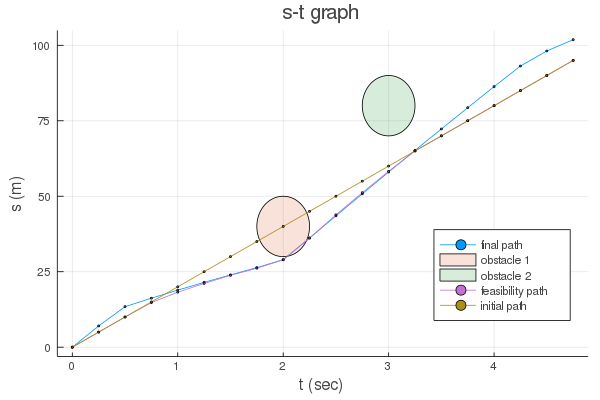
\includegraphics[scale=0.25]{img/path1d_interior1_st_test1}
\par\end{center}

We try to avoid the whole uncertainty area, complying to the minimax
approach $\underset{x\in\mathcal{X}}{\min}\quad\underset{z\in\mathcal{Z}}{\max}\quad f\left(x,z\right).$
But if we can not avoid the full uncertainty area, we will remain
as far as possible from its center, via the Elastic Collision Avoidance
Model described previously. This Elastic Model strictly enforces dynamics
constraints but relaxes the safety distance as little as possible.

\section{Experiments}

The gihub repo is \href{https://github.com/PhilippeW83440/AA222_Project}{AA222-project}. 

\subsection{Solvers Benchmarks}
\begin{itemize}
\item Runtime: $\leq250$ ms for real time applicability
\item Feasibility constraints compliance: check safety \& dynamics constraints
\item Cost value: efficiency and comfort (lower cost function)
\end{itemize}
Accuracy is similar for all solvers. The difference is the runtime.

\begin{figure}[H]
\noindent 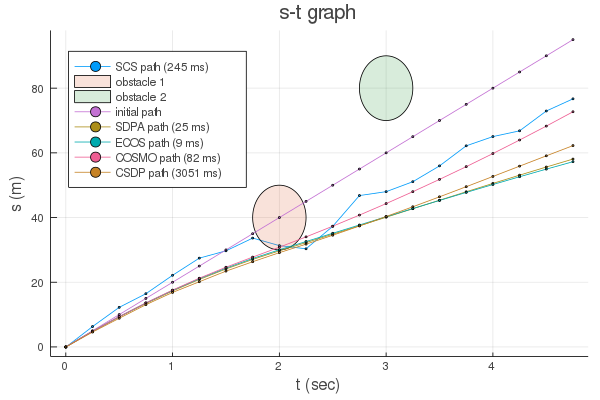
\includegraphics[scale=0.33]{img/st_graph_solvers}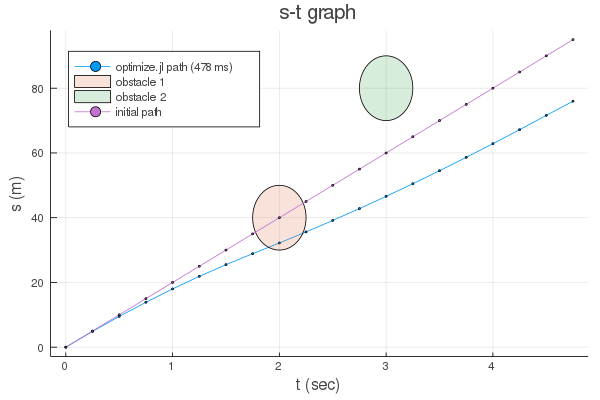
\includegraphics[scale=0.33]{img/path1d_interior_st_test2}

\caption{Solvers Runtime Benchmark}
\end{figure}

\begin{lstlisting}
MOSEK runtime=13 ms
Collision avoidance constraint 1: slack_col=3.19
Collision avoidance constraint 2: slack_col=-0.0
\end{lstlisting}

\begin{lstlisting}
OPTIMIZE.jl runtime=483 ms
Iter 124 BFGS=1.62 ms: INV=0.63 ms, BT=0.38 ms, GRAD=0.40 ms
max   equality constraint violation:(1.256239e-11, 4) out of 40
max inequality constraint violation:(-0.000311, 120) out of 122
Collision avoidance constraint: slack_col=[3.19, 0.0]
Pass: optimize returns a feasible solution on 2/2 random seeds.
\end{lstlisting}
\begin{center}
\par\end{center}

\subsection{Anti Collision Tests Benchmarks}

We use the MOSEK solver for these tests. While ECOS is even faster
in general, ECOS does not support Mixed Integer Programming which
we need for the most advanced version of the Collision Avoidance model.
MOSEK is a commercial solver for which we have an educational license.

We use five metrics to evaluate the performance of our different approaches.
$\left(1\right)$ The main success metric is the percentage of cases
where we reach a target state without collision. $\left(2\right)$
The second metric is the agent runtime. $\left(3\right)$ The third
metric is a comfort metric: the number of hard braking decisions.
$\left(4\right)$ The fourth metric relates to efficiency: how fast
we reach a target while complying to some speed limitation. $\left(5\right)$
The last metric is a safety metric: for some of our randomly generated
test cases, a collision is unavoidable. In these cases, we aim for
a lower speed at collision.

\begin{table}[H]
\centering{

\begin{tabular}{cccccc}
\toprule 
Mean & Success & Runtime & HardBrakes & Steps & Collision Speed\tabularnewline
\midrule
\midrule 
Baseline (Constant Speed) & 22\% & $<1\mu s$ & 0.0 & 40.0 & 20.0 m.s$^{-1}$\tabularnewline
\midrule 
MPC & 79\% & 19 ms & 3.09 & 39.5 & 18.5 m.s$^{-1}$\tabularnewline
\midrule 
MPC\_MIP & 96\% & 22 ms & 0.19 & 53.8 & 18.7 m.s$^{-1}$\tabularnewline
\midrule 
Oracle (Dynamic Programming) & 96\% & 22.3 sec & 0.48 & 33.1 & 15.5 m.s$^{-1}$\tabularnewline
\bottomrule
\end{tabular}

}

\caption{Results over 100 anti-collision tests}
\end{table}


\section{Conclusion }

We came up with a detailed analysis of a Trajectory Optimization problem.
We tackle the issue of Collision Avoidance of dynamic obstacles where
real-time decisions are required. We propose a Collision Avoidance
model based on an Elastic Model handling disjunctive constraints.
This solution is based on Mixed Integer Programming with core optimization
algorithms relying on primal-dual interior point methods. We also
investigate how the Simplex algorithm could be adapted to solve a
problem initially defined over a quadratic cost function. Finally
we demonstrate the efficiency of our proposed model, operating over
a continuous state space, with a runtime of $22$ ms. While being
$1000$ x faster than our Oracle, a Dynamic Programming implementation
performing an exhaustive search over a discretized solution space,
it achieves the same collision avoidance success rate.

\bibliographystyle{plain}
\nocite{*}
\bibliography{project}

\end{document}
